% Options for packages loaded elsewhere
\PassOptionsToPackage{unicode}{hyperref}
\PassOptionsToPackage{hyphens}{url}
%
\documentclass[
  11pt,
]{article}
\usepackage{lmodern}
\usepackage{amssymb,amsmath}
\usepackage{ifxetex,ifluatex}
\ifnum 0\ifxetex 1\fi\ifluatex 1\fi=0 % if pdftex
  \usepackage[T1]{fontenc}
  \usepackage[utf8]{inputenc}
  \usepackage{textcomp} % provide euro and other symbols
\else % if luatex or xetex
  \usepackage{unicode-math}
  \defaultfontfeatures{Scale=MatchLowercase}
  \defaultfontfeatures[\rmfamily]{Ligatures=TeX,Scale=1}
\fi
% Use upquote if available, for straight quotes in verbatim environments
\IfFileExists{upquote.sty}{\usepackage{upquote}}{}
\IfFileExists{microtype.sty}{% use microtype if available
  \usepackage[]{microtype}
  \UseMicrotypeSet[protrusion]{basicmath} % disable protrusion for tt fonts
}{}
\makeatletter
\@ifundefined{KOMAClassName}{% if non-KOMA class
  \IfFileExists{parskip.sty}{%
    \usepackage{parskip}
  }{% else
    \setlength{\parindent}{0pt}
    \setlength{\parskip}{6pt plus 2pt minus 1pt}}
}{% if KOMA class
  \KOMAoptions{parskip=half}}
\makeatother
\usepackage{xcolor}
\IfFileExists{xurl.sty}{\usepackage{xurl}}{} % add URL line breaks if available
\IfFileExists{bookmark.sty}{\usepackage{bookmark}}{\usepackage{hyperref}}
\hypersetup{
  pdftitle={Project 5},
  pdfauthor={Matt Wakefield},
  hidelinks,
  pdfcreator={LaTeX via pandoc}}
\urlstyle{same} % disable monospaced font for URLs
\usepackage[margin=1in]{geometry}
\usepackage{color}
\usepackage{fancyvrb}
\newcommand{\VerbBar}{|}
\newcommand{\VERB}{\Verb[commandchars=\\\{\}]}
\DefineVerbatimEnvironment{Highlighting}{Verbatim}{commandchars=\\\{\}}
% Add ',fontsize=\small' for more characters per line
\usepackage{framed}
\definecolor{shadecolor}{RGB}{248,248,248}
\newenvironment{Shaded}{\begin{snugshade}}{\end{snugshade}}
\newcommand{\AlertTok}[1]{\textcolor[rgb]{0.94,0.16,0.16}{#1}}
\newcommand{\AnnotationTok}[1]{\textcolor[rgb]{0.56,0.35,0.01}{\textbf{\textit{#1}}}}
\newcommand{\AttributeTok}[1]{\textcolor[rgb]{0.77,0.63,0.00}{#1}}
\newcommand{\BaseNTok}[1]{\textcolor[rgb]{0.00,0.00,0.81}{#1}}
\newcommand{\BuiltInTok}[1]{#1}
\newcommand{\CharTok}[1]{\textcolor[rgb]{0.31,0.60,0.02}{#1}}
\newcommand{\CommentTok}[1]{\textcolor[rgb]{0.56,0.35,0.01}{\textit{#1}}}
\newcommand{\CommentVarTok}[1]{\textcolor[rgb]{0.56,0.35,0.01}{\textbf{\textit{#1}}}}
\newcommand{\ConstantTok}[1]{\textcolor[rgb]{0.00,0.00,0.00}{#1}}
\newcommand{\ControlFlowTok}[1]{\textcolor[rgb]{0.13,0.29,0.53}{\textbf{#1}}}
\newcommand{\DataTypeTok}[1]{\textcolor[rgb]{0.13,0.29,0.53}{#1}}
\newcommand{\DecValTok}[1]{\textcolor[rgb]{0.00,0.00,0.81}{#1}}
\newcommand{\DocumentationTok}[1]{\textcolor[rgb]{0.56,0.35,0.01}{\textbf{\textit{#1}}}}
\newcommand{\ErrorTok}[1]{\textcolor[rgb]{0.64,0.00,0.00}{\textbf{#1}}}
\newcommand{\ExtensionTok}[1]{#1}
\newcommand{\FloatTok}[1]{\textcolor[rgb]{0.00,0.00,0.81}{#1}}
\newcommand{\FunctionTok}[1]{\textcolor[rgb]{0.00,0.00,0.00}{#1}}
\newcommand{\ImportTok}[1]{#1}
\newcommand{\InformationTok}[1]{\textcolor[rgb]{0.56,0.35,0.01}{\textbf{\textit{#1}}}}
\newcommand{\KeywordTok}[1]{\textcolor[rgb]{0.13,0.29,0.53}{\textbf{#1}}}
\newcommand{\NormalTok}[1]{#1}
\newcommand{\OperatorTok}[1]{\textcolor[rgb]{0.81,0.36,0.00}{\textbf{#1}}}
\newcommand{\OtherTok}[1]{\textcolor[rgb]{0.56,0.35,0.01}{#1}}
\newcommand{\PreprocessorTok}[1]{\textcolor[rgb]{0.56,0.35,0.01}{\textit{#1}}}
\newcommand{\RegionMarkerTok}[1]{#1}
\newcommand{\SpecialCharTok}[1]{\textcolor[rgb]{0.00,0.00,0.00}{#1}}
\newcommand{\SpecialStringTok}[1]{\textcolor[rgb]{0.31,0.60,0.02}{#1}}
\newcommand{\StringTok}[1]{\textcolor[rgb]{0.31,0.60,0.02}{#1}}
\newcommand{\VariableTok}[1]{\textcolor[rgb]{0.00,0.00,0.00}{#1}}
\newcommand{\VerbatimStringTok}[1]{\textcolor[rgb]{0.31,0.60,0.02}{#1}}
\newcommand{\WarningTok}[1]{\textcolor[rgb]{0.56,0.35,0.01}{\textbf{\textit{#1}}}}
\usepackage{longtable,booktabs}
% Correct order of tables after \paragraph or \subparagraph
\usepackage{etoolbox}
\makeatletter
\patchcmd\longtable{\par}{\if@noskipsec\mbox{}\fi\par}{}{}
\makeatother
% Allow footnotes in longtable head/foot
\IfFileExists{footnotehyper.sty}{\usepackage{footnotehyper}}{\usepackage{footnote}}
\makesavenoteenv{longtable}
\usepackage{graphicx,grffile}
\makeatletter
\def\maxwidth{\ifdim\Gin@nat@width>\linewidth\linewidth\else\Gin@nat@width\fi}
\def\maxheight{\ifdim\Gin@nat@height>\textheight\textheight\else\Gin@nat@height\fi}
\makeatother
% Scale images if necessary, so that they will not overflow the page
% margins by default, and it is still possible to overwrite the defaults
% using explicit options in \includegraphics[width, height, ...]{}
\setkeys{Gin}{width=\maxwidth,height=\maxheight,keepaspectratio}
% Set default figure placement to htbp
\makeatletter
\def\fps@figure{htbp}
\makeatother
\setlength{\emergencystretch}{3em} % prevent overfull lines
\providecommand{\tightlist}{%
  \setlength{\itemsep}{0pt}\setlength{\parskip}{0pt}}
\setcounter{secnumdepth}{-\maxdimen} % remove section numbering
\usepackage{amsmath}
\usepackage{amssymb}
\usepackage{amsfonts}
\usepackage{subfig}
\usepackage{graphicx}
\usepackage{amsthm}
\usepackage{fancyhdr}
\pagestyle{fancy}
\fancyhf{}
\rhead{STAT 5290-- Predictive Analytics}
\lhead{Project 5}
\cfoot{\thepage}
\usepackage{algorithm}
\usepackage[noend]{algpseudocode}

\title{Project 5}
\author{Matt Wakefield}
\date{May 05, 2021}

\begin{document}
\maketitle

{
\setcounter{tocdepth}{4}
\tableofcontents
}
\hypertarget{introduction.}{%
\subsection{Introduction.}\label{introduction.}}

Modeling climate change is an extraordinarily complex endevor that
require large disparate teams to contribute to the project according to
their area of expertise.

This model is developed via several parameters (columns 3 through 20).
Due to the complexity of this model it can crash at times. This is
represented by the outcome variable and contains the values 0 for
crashed or 1 for ran successfully.

The samples were gathered via a method known as latin hybercube
sampling. Which samples out of a cumulative density function where each
variable is it's own dimension.

Our goal will be to identify the parameters that are causing this
failure, and be able to accurately predict whether or not a series of
parameters will lead to a failure.

\hypertarget{data-preperation-and-exploratory-data-analysis}{%
\subsection{Data Preperation and Exploratory Data
Analysis}\label{data-preperation-and-exploratory-data-analysis}}

\begin{Shaded}
\begin{Highlighting}[]
\KeywordTok{library}\NormalTok{(tidyverse)}
\KeywordTok{library}\NormalTok{(skimr )}
\KeywordTok{library}\NormalTok{(corrplot)}
\KeywordTok{library}\NormalTok{(factoextra)}
\KeywordTok{library}\NormalTok{(ggfortify)}
\KeywordTok{library}\NormalTok{(tidymodels)}
\KeywordTok{library}\NormalTok{(keras)}
\KeywordTok{library}\NormalTok{(vip)}
\end{Highlighting}
\end{Shaded}

\hypertarget{read-file-and-present-basic-summary-data.}{%
\subsubsection{Read file and present basic summary
data.}\label{read-file-and-present-basic-summary-data.}}

\begin{Shaded}
\begin{Highlighting}[]
\NormalTok{df<-}\KeywordTok{read.table}\NormalTok{(}\StringTok{'http://archive.ics.uci.edu/ml/machine-learning-databases/00252/pop_failures.dat'}\NormalTok{, }\DataTypeTok{header =} \OtherTok{TRUE}\NormalTok{)}

\KeywordTok{skim_without_charts}\NormalTok{(df)}
\end{Highlighting}
\end{Shaded}

\begin{longtable}[]{@{}ll@{}}
\caption{Data summary}\tabularnewline
\toprule
\endhead
Name & df\tabularnewline
Number of rows & 540\tabularnewline
Number of columns & 21\tabularnewline
\_\_\_\_\_\_\_\_\_\_\_\_\_\_\_\_\_\_\_\_\_\_\_ &\tabularnewline
Column type frequency: &\tabularnewline
numeric & 21\tabularnewline
\_\_\_\_\_\_\_\_\_\_\_\_\_\_\_\_\_\_\_\_\_\_\_\_ &\tabularnewline
Group variables & None\tabularnewline
\bottomrule
\end{longtable}

\textbf{Variable type: numeric}

\begin{longtable}[]{@{}lrrrrrrrrr@{}}
\toprule
skim\_variable & n\_missing & complete\_rate & mean & sd & p0 & p25 &
p50 & p75 & p100\tabularnewline
\midrule
\endhead
Study & 0 & 1 & 2.00 & 0.82 & 1 & 1.00 & 2.0 & 3.00 & 3\tabularnewline
Run & 0 & 1 & 90.50 & 52.01 & 1 & 45.75 & 90.5 & 135.25 &
180\tabularnewline
vconst\_corr & 0 & 1 & 0.50 & 0.29 & 0 & 0.25 & 0.5 & 0.75 &
1\tabularnewline
vconst\_2 & 0 & 1 & 0.50 & 0.29 & 0 & 0.25 & 0.5 & 0.75 &
1\tabularnewline
vconst\_3 & 0 & 1 & 0.50 & 0.29 & 0 & 0.25 & 0.5 & 0.75 &
1\tabularnewline
vconst\_4 & 0 & 1 & 0.50 & 0.29 & 0 & 0.25 & 0.5 & 0.75 &
1\tabularnewline
vconst\_5 & 0 & 1 & 0.50 & 0.29 & 0 & 0.25 & 0.5 & 0.75 &
1\tabularnewline
vconst\_7 & 0 & 1 & 0.50 & 0.29 & 0 & 0.25 & 0.5 & 0.75 &
1\tabularnewline
ah\_corr & 0 & 1 & 0.50 & 0.29 & 0 & 0.25 & 0.5 & 0.75 &
1\tabularnewline
ah\_bolus & 0 & 1 & 0.50 & 0.29 & 0 & 0.25 & 0.5 & 0.75 &
1\tabularnewline
slm\_corr & 0 & 1 & 0.50 & 0.29 & 0 & 0.25 & 0.5 & 0.75 &
1\tabularnewline
efficiency\_factor & 0 & 1 & 0.50 & 0.29 & 0 & 0.25 & 0.5 & 0.75 &
1\tabularnewline
tidal\_mix\_max & 0 & 1 & 0.50 & 0.29 & 0 & 0.25 & 0.5 & 0.75 &
1\tabularnewline
vertical\_decay\_scale & 0 & 1 & 0.50 & 0.29 & 0 & 0.25 & 0.5 & 0.75 &
1\tabularnewline
convect\_corr & 0 & 1 & 0.50 & 0.29 & 0 & 0.25 & 0.5 & 0.75 &
1\tabularnewline
bckgrnd\_vdc1 & 0 & 1 & 0.50 & 0.29 & 0 & 0.25 & 0.5 & 0.75 &
1\tabularnewline
bckgrnd\_vdc\_ban & 0 & 1 & 0.50 & 0.29 & 0 & 0.25 & 0.5 & 0.75 &
1\tabularnewline
bckgrnd\_vdc\_eq & 0 & 1 & 0.50 & 0.29 & 0 & 0.25 & 0.5 & 0.75 &
1\tabularnewline
bckgrnd\_vdc\_psim & 0 & 1 & 0.50 & 0.29 & 0 & 0.25 & 0.5 & 0.75 &
1\tabularnewline
Prandtl & 0 & 1 & 0.50 & 0.29 & 0 & 0.25 & 0.5 & 0.75 & 1\tabularnewline
outcome & 0 & 1 & 0.91 & 0.28 & 0 & 1.00 & 1.0 & 1.00 & 1\tabularnewline
\bottomrule
\end{longtable}

Firstly we observe that there are no missing values, thus there's no
need for imputation.

What we can observe is that each of the variables has been normalized at
a scale of 0 to 1, with each ntile corresponding the value (e.g.~.25
corresponds to the 25th percentile)

The first and second variables, Study and Run, are likely not relevant
to the outcome. Through EDA we can at least gauge whether or not Study
is equally representative.

Most of the focus of the EDA will be on how the variables relate to one
another, and if it's immediately apparent that these variables appear to
be associated with failures.

\hypertarget{correlation-among-variables}{%
\subsubsection{Correlation Among
Variables}\label{correlation-among-variables}}

\begin{Shaded}
\begin{Highlighting}[]
\NormalTok{df_corr<-df}\OperatorTok\KeywordTok{select}\NormalTok{(}\OperatorTok{-}\KeywordTok{c}\NormalTok{(Study, Run, outcome))}\OperatorTok\KeywordTok{cor}\NormalTok{()}
\KeywordTok{corrplot}\NormalTok{(df_corr, }\DataTypeTok{type=}\StringTok{"upper"}\NormalTok{,}\DataTypeTok{method =} \StringTok{"color"}\NormalTok{, }\DataTypeTok{add.coef.col =} \StringTok{'black'}\NormalTok{,}\DataTypeTok{tl.col =} \StringTok{'black'}\NormalTok{,}\DataTypeTok{number.cex=} \FloatTok{.5}\NormalTok{, }\DataTypeTok{tl.cex =} \FloatTok{.6}\NormalTok{)}
\end{Highlighting}
\end{Shaded}

\begin{verbatim}
## Warning in text.default(pos.xlabel[, 1], pos.xlabel[, 2], newcolnames, srt =
## tl.srt, : "add.coef.col" is not a graphical parameter
\end{verbatim}

\begin{verbatim}
## Warning in text.default(pos.ylabel[, 1], pos.ylabel[, 2], newrownames, col =
## tl.col, : "add.coef.col" is not a graphical parameter
\end{verbatim}

\begin{verbatim}
## Warning in title(title, ...): "add.coef.col" is not a graphical parameter
\end{verbatim}

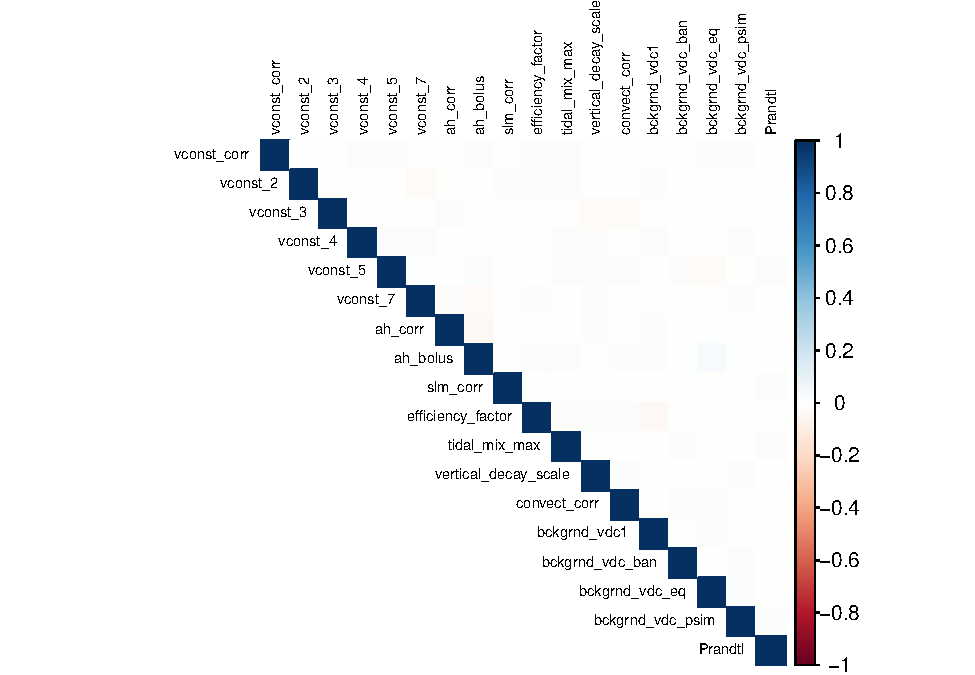
\includegraphics{Project-5-MTW_files/figure-latex/unnamed-chunk-3-1.pdf}

\begin{Shaded}
\begin{Highlighting}[]
\KeywordTok{paste}\NormalTok{(}\StringTok{'The Average Correlation is'}\NormalTok{, df_corr[df_corr }\OperatorTok{!=}\DecValTok{1}\NormalTok{]}\OperatorTok\KeywordTok{mean}\NormalTok{()}\OperatorTok\KeywordTok{round}\NormalTok{(.,}\DecValTok{5}\NormalTok{))}
\end{Highlighting}
\end{Shaded}

\begin{verbatim}
## [1] "The Average Correlation is 0.00025"
\end{verbatim}

Perhaps as a result of the normalization effort somehow leads to 0
correlation. Regardless, we can assume that our variables are about as
independent as possible.

\hypertarget{principal-component-analysis}{%
\subsubsection{Principal Component
Analysis}\label{principal-component-analysis}}

\begin{Shaded}
\begin{Highlighting}[]
\KeywordTok{par}\NormalTok{(}\DataTypeTok{mar =} \KeywordTok{c}\NormalTok{(}\DecValTok{0}\NormalTok{, }\DecValTok{0}\NormalTok{, }\DecValTok{0}\NormalTok{, }\DecValTok{0}\NormalTok{))}
\NormalTok{df_pca<-df}\OperatorTok\KeywordTok{select}\NormalTok{(}\OperatorTok{-}\KeywordTok{c}\NormalTok{(Study, Run, outcome))}\OperatorTok\KeywordTok{as.matrix}\NormalTok{()}
\NormalTok{df_pca <-}\StringTok{ }\KeywordTok{prcomp}\NormalTok{(df_pca, }\DataTypeTok{scale =} \OtherTok{TRUE}\NormalTok{, }\DataTypeTok{center =} \OtherTok{TRUE}\NormalTok{)}
\NormalTok{pca_viz<-}\KeywordTok{fviz_eig}\NormalTok{(df_pca, }\DataTypeTok{ncp =} \DecValTok{18}\NormalTok{)}
\NormalTok{pca_viz}
\end{Highlighting}
\end{Shaded}

\begin{flushleft}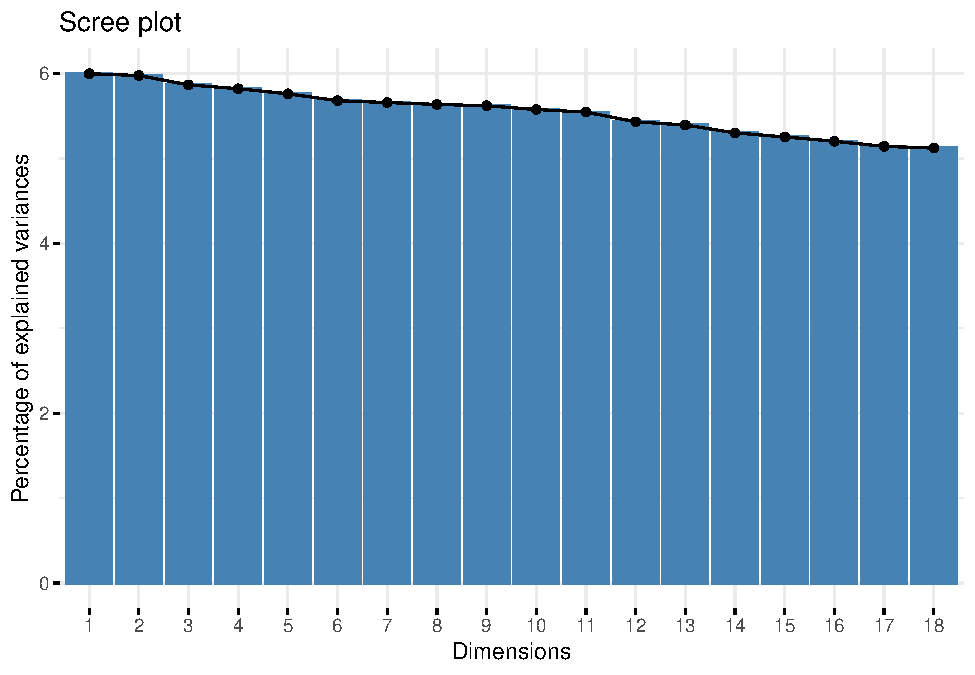
\includegraphics{Project-5-MTW_files/figure-latex/unnamed-chunk-4-1} \end{flushleft}

As we can see, each additional PCA dimension consistently adds between 5
and 6 percent variance. Typically want we want to see is that one
particular dimension is clearly in the lead, so we can list those
variables to see what's really influencing the shape of this data.

Regardless the 1st PCA is listed below:

\begin{Shaded}
\begin{Highlighting}[]
\NormalTok{df_pca}\OperatorTok{$}\NormalTok{rotation[,}\DecValTok{1}\NormalTok{]}\OperatorTok\KeywordTok{abs}\NormalTok{()}\OperatorTok\KeywordTok{sort}\NormalTok{(., }\DataTypeTok{decreasing =}\NormalTok{ T)}\OperatorTok\KeywordTok{head}\NormalTok{(}\DecValTok{4}\NormalTok{)}
\end{Highlighting}
\end{Shaded}

\begin{verbatim}
## bckgrnd_vdc_eq       vconst_5       ah_bolus       vconst_4 
##      0.4540322      0.3886978      0.3774293      0.3288626
\end{verbatim}

\begin{Shaded}
\begin{Highlighting}[]
\KeywordTok{autoplot}\NormalTok{(df_pca, }\DataTypeTok{data =}\NormalTok{ df, }\DataTypeTok{colour =} \StringTok{'outcome'}\NormalTok{,}
         \DataTypeTok{loadings =} \OtherTok{TRUE}\NormalTok{, }\DataTypeTok{loadings.colour =} \StringTok{'blue'}\NormalTok{,}
         \DataTypeTok{loadings.label =} \OtherTok{TRUE}\NormalTok{, }\DataTypeTok{loadings.label.size =} \DecValTok{3}\NormalTok{)}
\end{Highlighting}
\end{Shaded}

\begin{verbatim}
## Warning: `select_()` was deprecated in dplyr 0.7.0.
## Please use `select()` instead.
\end{verbatim}

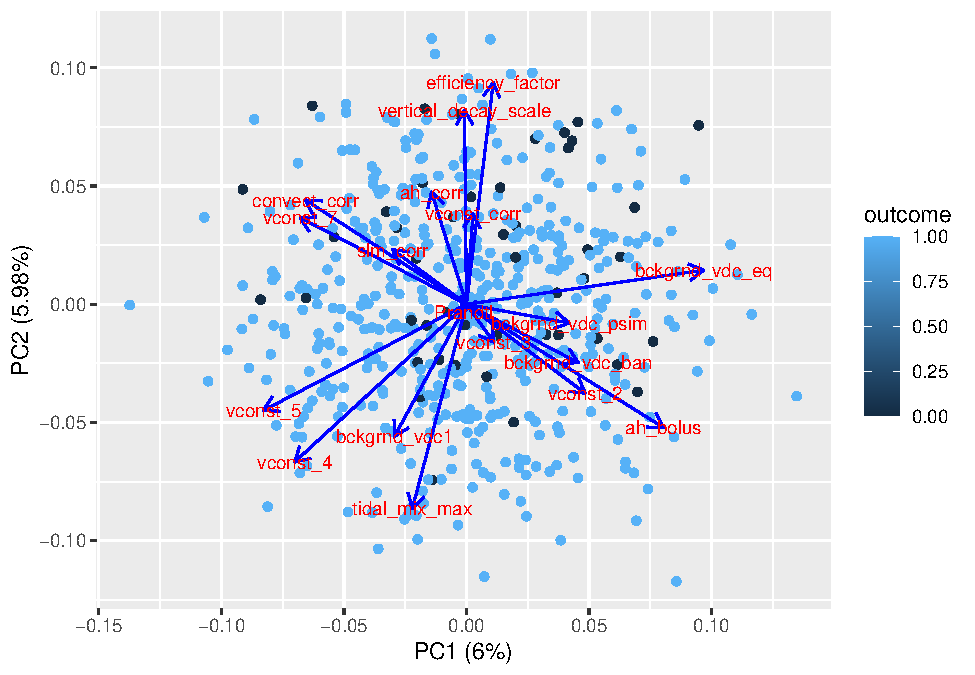
\includegraphics{Project-5-MTW_files/figure-latex/unnamed-chunk-6-1.pdf}

As we can see the variables are all over the place, as is the relation
of those variables to the outcome. One possible trend is in the lower
right hand side of the plot, that indicates ah\_bolus, vconst\_2,
v\_const3, backgrnd\_vdc\_ban, and backgrnd\_vdc\_psim all vary together
somewhat. Unfortunately the scattering of outcomes is just as random as
it is across the rest of the plot, and the overall contribution to
variance is still very small.

The PCA does not give us a clear idea of variables we can discard yet to
encourage a parsimonious model.

\hypertarget{means-of-values-related-to-failure.}{%
\subsubsection{Means of values related to
failure.}\label{means-of-values-related-to-failure.}}

\begin{Shaded}
\begin{Highlighting}[]
\NormalTok{df_means<-df}\OperatorTok\KeywordTok{select}\NormalTok{(}\OperatorTok{-}\KeywordTok{c}\NormalTok{(Study, Run))}
\NormalTok{df_means<-df_means}\OperatorTok\KeywordTok{pivot_longer}\NormalTok{(}\DataTypeTok{cols =} \OperatorTok{-}\KeywordTok{c}\NormalTok{(outcome))}\OperatorTok\KeywordTok{group_by}\NormalTok{(outcome, name)}\OperatorTok\KeywordTok{summarise}\NormalTok{(}\DataTypeTok{mean =} \KeywordTok{mean}\NormalTok{(value))}\OperatorTok\KeywordTok{filter}\NormalTok{(outcome }\OperatorTok{==}\StringTok{ }\DecValTok{0}\NormalTok{)}\OperatorTok\KeywordTok{arrange}\NormalTok{(}\KeywordTok{desc}\NormalTok{(mean))}
\NormalTok{df_means}
\end{Highlighting}
\end{Shaded}

\begin{verbatim}
## # A tibble: 18 x 3
## # Groups:   outcome [1]
##    outcome name                  mean
##      <int> <chr>                <dbl>
##  1       0 vconst_corr          0.788
##  2       0 vconst_2             0.786
##  3       0 convect_corr         0.682
##  4       0 vertical_decay_scale 0.543
##  5       0 efficiency_factor    0.531
##  6       0 bckgrnd_vdc_ban      0.527
##  7       0 Prandtl              0.526
##  8       0 tidal_mix_max        0.514
##  9       0 vconst_3             0.500
## 10       0 ah_bolus             0.496
## 11       0 ah_corr              0.484
## 12       0 vconst_7             0.454
## 13       0 slm_corr             0.454
## 14       0 vconst_5             0.449
## 15       0 bckgrnd_vdc_psim     0.445
## 16       0 vconst_4             0.432
## 17       0 bckgrnd_vdc_eq       0.426
## 18       0 bckgrnd_vdc1         0.326
\end{verbatim}

We finally have some hints about how this data may be related to
failure.

Because the data has been normalized, we can compare the mean of one
variable to another. Note that the mean value of vconst\_corr is much
higher for failures (.78) then it is bckgrnd\_vdc1 (.33)

Perhaps the model that creates this variable should be looked at to see
why higher values would cause a crash.

\begin{Shaded}
\begin{Highlighting}[]
\KeywordTok{table}\NormalTok{(df}\OperatorTok{$}\NormalTok{outcome)}
\end{Highlighting}
\end{Shaded}

\begin{verbatim}
## 
##   0   1 
##  46 494
\end{verbatim}

Finally we can see that we are dealing with a very imbalanced target
variable. With the ratio of the majority being over 10x that of the
minority.

\hypertarget{data-partition}{%
\subsection{Data Partition}\label{data-partition}}

\begin{Shaded}
\begin{Highlighting}[]
\KeywordTok{set.seed}\NormalTok{(}\DecValTok{123}\NormalTok{)}

\NormalTok{df<-df}\OperatorTok\KeywordTok{select}\NormalTok{(}\OperatorTok{-}\KeywordTok{c}\NormalTok{(Study,Run))}

\NormalTok{df}\OperatorTok{$}\NormalTok{outcome<-df}\OperatorTok{$}\NormalTok{outcome}\OperatorTok\KeywordTok{factor}\NormalTok{()}
\NormalTok{n <-}\StringTok{ }\KeywordTok{nrow}\NormalTok{(df)}
\NormalTok{split_data <-}\StringTok{ }\KeywordTok{sample}\NormalTok{(}\DataTypeTok{x=}\DecValTok{1}\OperatorTok{:}\DecValTok{2}\NormalTok{, }\DataTypeTok{size =}\NormalTok{ n, }\DataTypeTok{replace=}\OtherTok{TRUE}\NormalTok{, }\DataTypeTok{prob=}\KeywordTok{c}\NormalTok{(}\FloatTok{0.67}\NormalTok{, }\FloatTok{0.33}\NormalTok{))}
\NormalTok{D1 <-}\StringTok{ }\NormalTok{df[split_data }\OperatorTok{==}\StringTok{ }\DecValTok{1}\NormalTok{, ]}
\NormalTok{D2 <-}\StringTok{ }\NormalTok{df[split_data }\OperatorTok{==}\StringTok{ }\DecValTok{2}\NormalTok{, ]}
\NormalTok{y.train <-}\StringTok{ }\NormalTok{D1}\OperatorTok{$}\NormalTok{outcome}
\NormalTok{yobs <-}\StringTok{ }\NormalTok{D2}\OperatorTok{$}\NormalTok{outcome}

\KeywordTok{data.frame}\NormalTok{(}\StringTok{'Split'}\NormalTok{=}\KeywordTok{c}\NormalTok{(}\StringTok{'Train'}\NormalTok{,}\StringTok{'Test'}\NormalTok{),}\StringTok{'Observations'}\NormalTok{=}\KeywordTok{c}\NormalTok{(}\KeywordTok{nrow}\NormalTok{(D1), }\KeywordTok{nrow}\NormalTok{(D2)))}
\end{Highlighting}
\end{Shaded}

\begin{verbatim}
##   Split Observations
## 1 Train          367
## 2  Test          173
\end{verbatim}

Due to class imbalance of the target variable, let's go ahead and
upsample the training set.

\begin{Shaded}
\begin{Highlighting}[]
\NormalTok{D1_upsample <-}\StringTok{ }\KeywordTok{recipe}\NormalTok{( }\OperatorTok{~}\StringTok{ }\NormalTok{., }\DataTypeTok{data =}\NormalTok{ D1) }\OperatorTok
\StringTok{  }\KeywordTok{step_upsample}\NormalTok{(outcome, }\DataTypeTok{over_ratio =}\NormalTok{ (}\DecValTok{1}\OperatorTok{/}\DecValTok{3}\NormalTok{))}\OperatorTok
\StringTok{  }\KeywordTok{prep}\NormalTok{(}\DataTypeTok{training =}\NormalTok{ D1)}
\end{Highlighting}
\end{Shaded}

\begin{verbatim}
## Warning: `step_upsample()` was deprecated in recipes 0.1.13.
## Please use `themis::step_upsample()` instead.
\end{verbatim}

\begin{Shaded}
\begin{Highlighting}[]
\NormalTok{D1 <-}\StringTok{ }\KeywordTok{bake}\NormalTok{(D1_upsample, }\DataTypeTok{new_data =} \OtherTok{NULL}\NormalTok{)}

\KeywordTok{table}\NormalTok{(D1}\OperatorTok{$}\NormalTok{outcome)}
\end{Highlighting}
\end{Shaded}

\begin{verbatim}
## 
##   0   1 
## 112 336
\end{verbatim}

\hypertarget{models}{%
\subsection{Models}\label{models}}

\hypertarget{logistic-regression}{%
\subsubsection{Logistic Regression}\label{logistic-regression}}

\begin{Shaded}
\begin{Highlighting}[]
\NormalTok{log_mod<-}\KeywordTok{logistic_reg}\NormalTok{(}\DataTypeTok{penalty =} \KeywordTok{tune}\NormalTok{(), }\DataTypeTok{mixture =} \KeywordTok{tune}\NormalTok{())}\OperatorTok
\StringTok{  }\KeywordTok{set_engine}\NormalTok{(}\StringTok{'glmnet'}\NormalTok{)}\OperatorTok
\StringTok{  }\KeywordTok{set_mode}\NormalTok{(}\StringTok{'classification'}\NormalTok{)}

\NormalTok{log_grid<-}\KeywordTok{grid_regular}\NormalTok{(}\KeywordTok{penalty}\NormalTok{(),}\KeywordTok{mixture}\NormalTok{(),}\DataTypeTok{levels =} \DecValTok{20}\NormalTok{)}

\NormalTok{D1_folds<-}\KeywordTok{vfold_cv}\NormalTok{(D1)}

\NormalTok{log_wf<-}\KeywordTok{workflow}\NormalTok{()}\OperatorTok
\StringTok{  }\KeywordTok{add_model}\NormalTok{(log_mod)}\OperatorTok
\StringTok{  }\KeywordTok{add_formula}\NormalTok{(outcome }\OperatorTok{~}\StringTok{ }\NormalTok{.)}

\NormalTok{log_res<-log_wf}\OperatorTok\KeywordTok{tune_grid}\NormalTok{(}\DataTypeTok{resamples =}\NormalTok{ D1_folds,}
                              \DataTypeTok{grid =}\NormalTok{ log_grid)}
\end{Highlighting}
\end{Shaded}

\begin{verbatim}
## Warning: package 'rlang' was built under R version 4.0.5
\end{verbatim}

\begin{verbatim}
## Warning: package 'vctrs' was built under R version 4.0.5
\end{verbatim}

\begin{verbatim}
## Warning: package 'glmnet' was built under R version 4.0.4
\end{verbatim}

\begin{Shaded}
\begin{Highlighting}[]
\NormalTok{log_best<-log_res}\OperatorTok\KeywordTok{select_best}\NormalTok{(}\StringTok{"roc_auc"}\NormalTok{)}

\NormalTok{final_log_wf<-log_wf}\OperatorTok\KeywordTok{finalize_workflow}\NormalTok{(log_best)}

\NormalTok{final_log<-final_log_wf}\OperatorTok\KeywordTok{fit}\NormalTok{(}\DataTypeTok{data =}\NormalTok{ D1)}

\NormalTok{final_log}\OperatorTok{$}\NormalTok{fit}\OperatorTok{$}\NormalTok{fit}\OperatorTok{$}\NormalTok{spec}
\end{Highlighting}
\end{Shaded}

\begin{verbatim}
## Logistic Regression Model Specification (classification)
## 
## Main Arguments:
##   penalty = 0.00233572146909012
##   mixture = 0.684210526315789
## 
## Computational engine: glmnet 
## 
## Model fit template:
## glmnet::glmnet(x = missing_arg(), y = missing_arg(), weights = missing_arg(), 
##     alpha = 0.684210526315789, family = "binomial")
\end{verbatim}

\begin{Shaded}
\begin{Highlighting}[]
\NormalTok{ final_log}\OperatorTok
\StringTok{  }\KeywordTok{pull_workflow_fit}\NormalTok{() }\OperatorTok
\StringTok{  }\KeywordTok{tidy}\NormalTok{()}
\end{Highlighting}
\end{Shaded}

\begin{verbatim}
## # A tibble: 19 x 3
##    term                 estimate penalty
##    <chr>                   <dbl>   <dbl>
##  1 (Intercept)           21.4    0.00234
##  2 vconst_corr          -13.0    0.00234
##  3 vconst_2             -11.8    0.00234
##  4 vconst_3              -1.45   0.00234
##  5 vconst_4              -0.204  0.00234
##  6 vconst_5               1.03   0.00234
##  7 vconst_7               0      0.00234
##  8 ah_corr                0.479  0.00234
##  9 ah_bolus              -2.39   0.00234
## 10 slm_corr              -0.0961 0.00234
## 11 efficiency_factor     -1.67   0.00234
## 12 tidal_mix_max         -1.61   0.00234
## 13 vertical_decay_scale  -1.34   0.00234
## 14 convect_corr          -5.72   0.00234
## 15 bckgrnd_vdc1           5.88   0.00234
## 16 bckgrnd_vdc_ban        1.22   0.00234
## 17 bckgrnd_vdc_eq         1.17   0.00234
## 18 bckgrnd_vdc_psim       1.13   0.00234
## 19 Prandtl                0.410  0.00234
\end{verbatim}

\begin{Shaded}
\begin{Highlighting}[]
\NormalTok{prediction_metrics_log<-}\KeywordTok{data.frame}\NormalTok{(D2}\OperatorTok{$}\NormalTok{outcome,}\KeywordTok{predict}\NormalTok{(final_log,D2),}\KeywordTok{predict}\NormalTok{(final_log,D2, }\DataTypeTok{type =} \StringTok{"prob"}\NormalTok{))}

\NormalTok{metrics_log<-}\KeywordTok{metrics}\NormalTok{(prediction_metrics_log, D2.outcome,.pred_class, .pred_}\DecValTok{0}\NormalTok{)}

\NormalTok{metrics<-}\KeywordTok{data.frame}\NormalTok{(}\DataTypeTok{Model_Type=}\StringTok{'Logistic_Model'}\NormalTok{,metrics_log)}
\end{Highlighting}
\end{Shaded}

Here we are using an elastic net that is closer to ridge regression then
it is lasso regression. These parameters were chosen via a grid search
of 20 samples using 10 fold cross validation.

\begin{Shaded}
\begin{Highlighting}[]
\NormalTok{final_log}\OperatorTok
\StringTok{    }\KeywordTok{pull_workflow_fit}\NormalTok{() }\OperatorTok
\StringTok{    }\KeywordTok{tidy}\NormalTok{()}\OperatorTok\KeywordTok{arrange}\NormalTok{(}\KeywordTok{desc}\NormalTok{(}\KeywordTok{abs}\NormalTok{(estimate)))}
\end{Highlighting}
\end{Shaded}

\begin{verbatim}
## # A tibble: 19 x 3
##    term                 estimate penalty
##    <chr>                   <dbl>   <dbl>
##  1 (Intercept)           21.4    0.00234
##  2 vconst_corr          -13.0    0.00234
##  3 vconst_2             -11.8    0.00234
##  4 bckgrnd_vdc1           5.88   0.00234
##  5 convect_corr          -5.72   0.00234
##  6 ah_bolus              -2.39   0.00234
##  7 efficiency_factor     -1.67   0.00234
##  8 tidal_mix_max         -1.61   0.00234
##  9 vconst_3              -1.45   0.00234
## 10 vertical_decay_scale  -1.34   0.00234
## 11 bckgrnd_vdc_ban        1.22   0.00234
## 12 bckgrnd_vdc_eq         1.17   0.00234
## 13 bckgrnd_vdc_psim       1.13   0.00234
## 14 vconst_5               1.03   0.00234
## 15 ah_corr                0.479  0.00234
## 16 Prandtl                0.410  0.00234
## 17 vconst_4              -0.204  0.00234
## 18 slm_corr              -0.0961 0.00234
## 19 vconst_7               0      0.00234
\end{verbatim}

Above indicates the magnitude of the coefficients. Because all variables
were normalized beforehand, we can safely assume that the largest
absolute value of the coefficient is a pretty good indicator of variable
importance.

\hypertarget{random-forest}{%
\subsubsection{Random Forest}\label{random-forest}}

\begin{Shaded}
\begin{Highlighting}[]
\NormalTok{rf_mod<-}\KeywordTok{rand_forest}\NormalTok{(}\DataTypeTok{mtry =}\KeywordTok{tune}\NormalTok{(),}\DataTypeTok{trees =} \KeywordTok{tune}\NormalTok{(), }\DataTypeTok{min_n =} \KeywordTok{tune}\NormalTok{())}\OperatorTok
\StringTok{  }\KeywordTok{set_engine}\NormalTok{(}\StringTok{'ranger'}\NormalTok{,}\DataTypeTok{importance =} \StringTok{"permutation"}\NormalTok{)}\OperatorTok
\CommentTok{#%>%}
\StringTok{  }\KeywordTok{set_mode}\NormalTok{(}\StringTok{'classification'}\NormalTok{)}


\NormalTok{rf_wf<-}\KeywordTok{workflow}\NormalTok{()}\OperatorTok
\StringTok{  }\KeywordTok{add_model}\NormalTok{(rf_mod)}\OperatorTok
\StringTok{  }\KeywordTok{add_formula}\NormalTok{(outcome }\OperatorTok{~}\StringTok{ }\NormalTok{.)}

\CommentTok{#rf_res<-rf_wf%>%tune_grid(resamples = D1_folds,}
\CommentTok{#                              grid = rf_grid)}

\NormalTok{rf_res<-rf_wf}\OperatorTok\KeywordTok{tune_grid}\NormalTok{(}\DataTypeTok{resamples =}\NormalTok{ D1_folds,}
                              \DataTypeTok{grid =} \DecValTok{20}\NormalTok{)}
\end{Highlighting}
\end{Shaded}

\begin{verbatim}
## i Creating pre-processing data to finalize unknown parameter: mtry
\end{verbatim}

\begin{verbatim}
## Warning: package 'ranger' was built under R version 4.0.5
\end{verbatim}

\begin{Shaded}
\begin{Highlighting}[]
\NormalTok{rf_best<-rf_res}\OperatorTok\KeywordTok{select_best}\NormalTok{(}\StringTok{"roc_auc"}\NormalTok{)}

\NormalTok{final_rf_wf<-rf_wf}\OperatorTok\KeywordTok{finalize_workflow}\NormalTok{(rf_best)}

\NormalTok{final_rf<-final_rf_wf}\OperatorTok\KeywordTok{fit}\NormalTok{(}\DataTypeTok{data =}\NormalTok{ D1)}
\end{Highlighting}
\end{Shaded}

Similar to our log model process, we run a grid pattern of 20 values for
trees and min\_n.

\begin{Shaded}
\begin{Highlighting}[]
\NormalTok{final_rf}\OperatorTok
\StringTok{    }\KeywordTok{pull_workflow_fit}\NormalTok{() }\OperatorTok
\StringTok{    }\KeywordTok{vip}\NormalTok{(}\DataTypeTok{geom =} \StringTok{"col"}\NormalTok{)}
\end{Highlighting}
\end{Shaded}

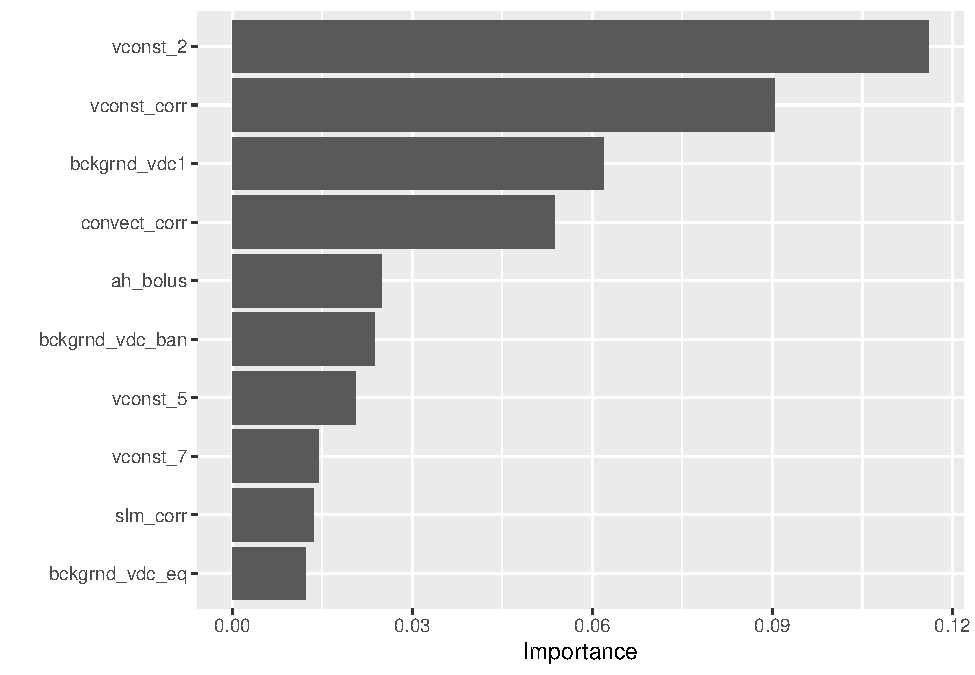
\includegraphics{Project-5-MTW_files/figure-latex/unnamed-chunk-14-1.pdf}

\begin{Shaded}
\begin{Highlighting}[]
\NormalTok{prediction_metrics_rf<-}\KeywordTok{data.frame}\NormalTok{(D2}\OperatorTok{$}\NormalTok{outcome,}\KeywordTok{predict}\NormalTok{(final_rf,D2),}\KeywordTok{predict}\NormalTok{(final_rf,D2, }\DataTypeTok{type =} \StringTok{"prob"}\NormalTok{))}

\NormalTok{metrics_rf<-}\KeywordTok{metrics}\NormalTok{(prediction_metrics_rf, D2.outcome,.pred_class, .pred_}\DecValTok{0}\NormalTok{)}

\NormalTok{metrics<-}\KeywordTok{rbind}\NormalTok{(metrics,}\KeywordTok{data.frame}\NormalTok{(}\DataTypeTok{Model_Type=}\StringTok{'Random_Forest'}\NormalTok{,metrics_rf))}
\end{Highlighting}
\end{Shaded}

As we can see, the importance of the factors is similar to the log model
as well with vconst\_2 and vconst\_corr pulling well ahead of the
others.

\hypertarget{neural-nets}{%
\subsubsection{Neural Nets}\label{neural-nets}}

\begin{Shaded}
\begin{Highlighting}[]
\NormalTok{D1_x<-D1}\OperatorTok\KeywordTok{select}\NormalTok{(}\OperatorTok{-}\NormalTok{outcome)}\OperatorTok\KeywordTok{as.matrix}\NormalTok{()}
\NormalTok{D1_y<-D1}\OperatorTok\KeywordTok{select}\NormalTok{(outcome)}\OperatorTok\KeywordTok{as.matrix}\NormalTok{()}\OperatorTok\KeywordTok{to_categorical}\NormalTok{()}

\NormalTok{D2_x<-D2}\OperatorTok\KeywordTok{select}\NormalTok{(}\OperatorTok{-}\NormalTok{outcome)}\OperatorTok\KeywordTok{as.matrix}\NormalTok{()}
\NormalTok{D2_y<-D2}\OperatorTok\KeywordTok{select}\NormalTok{(outcome)}\OperatorTok\KeywordTok{as.matrix}\NormalTok{()}\OperatorTok\KeywordTok{to_categorical}\NormalTok{()}

\NormalTok{nn_mod<-}\KeywordTok{mlp}\NormalTok{(}\DataTypeTok{hidden_units =} \KeywordTok{c}\NormalTok{(}\DecValTok{4}\NormalTok{,}\DecValTok{2}\NormalTok{))}\OperatorTok
\StringTok{  }\KeywordTok{set_engine}\NormalTok{(}\StringTok{'nnet'}\NormalTok{)}\OperatorTok
\StringTok{  }\KeywordTok{set_mode}\NormalTok{(}\StringTok{'classification'}\NormalTok{)}

\NormalTok{nn_mod2 <-}\StringTok{ }\KeywordTok{keras_model_sequential}\NormalTok{() }\OperatorTok
\StringTok{  }\KeywordTok{layer_dense}\NormalTok{(}\DataTypeTok{units =} \DecValTok{10}\NormalTok{, }\DataTypeTok{activation =} \StringTok{"relu"}\NormalTok{, }\DataTypeTok{input_shape =} \DecValTok{18}\NormalTok{) }\OperatorTok
\StringTok{  }\KeywordTok{layer_dense}\NormalTok{(}\DataTypeTok{units =} \DecValTok{30}\NormalTok{, }\DataTypeTok{activation =} \StringTok{"relu"}\NormalTok{) }\OperatorTok
\StringTok{  }\KeywordTok{layer_dense}\NormalTok{(}\DataTypeTok{units =} \DecValTok{2}\NormalTok{, }\DataTypeTok{activation =} \StringTok{"sigmoid"}\NormalTok{)}\OperatorTok
\StringTok{  }\KeywordTok{compile}\NormalTok{(}
    \DataTypeTok{loss =} \StringTok{'categorical_crossentropy'}\NormalTok{,}
    \DataTypeTok{optimizer =} \KeywordTok{optimizer_rmsprop}\NormalTok{(),}
    \DataTypeTok{metrics =} \KeywordTok{c}\NormalTok{(}\StringTok{'accuracy'}\NormalTok{)}
\NormalTok{  )}


\NormalTok{nn_mod4 <-}\StringTok{ }\KeywordTok{keras_model_sequential}\NormalTok{() }\OperatorTok
\StringTok{  }\KeywordTok{layer_dense}\NormalTok{(}\DataTypeTok{units =} \DecValTok{10}\NormalTok{, }\DataTypeTok{activation =} \StringTok{"relu"}\NormalTok{, }\DataTypeTok{input_shape =} \DecValTok{18}\NormalTok{) }\OperatorTok
\StringTok{  }\KeywordTok{layer_dense}\NormalTok{(}\DataTypeTok{units =} \DecValTok{30}\NormalTok{, }\DataTypeTok{activation =} \StringTok{"relu"}\NormalTok{) }\OperatorTok
\StringTok{    }\KeywordTok{layer_dense}\NormalTok{(}\DataTypeTok{units =} \DecValTok{75}\NormalTok{, }\DataTypeTok{activation =} \StringTok{"relu"}\NormalTok{) }\OperatorTok
\StringTok{    }\KeywordTok{layer_dense}\NormalTok{(}\DataTypeTok{units =} \DecValTok{40}\NormalTok{, }\DataTypeTok{activation =} \StringTok{"relu"}\NormalTok{) }\OperatorTok
\StringTok{  }\KeywordTok{layer_dense}\NormalTok{(}\DataTypeTok{units =} \DecValTok{2}\NormalTok{, }\DataTypeTok{activation =} \StringTok{"sigmoid"}\NormalTok{)}\OperatorTok
\StringTok{  }\KeywordTok{compile}\NormalTok{(}
    \DataTypeTok{loss =} \StringTok{'categorical_crossentropy'}\NormalTok{,}
    \DataTypeTok{optimizer =} \KeywordTok{optimizer_rmsprop}\NormalTok{(),}
    \DataTypeTok{metrics =} \KeywordTok{c}\NormalTok{(}\StringTok{'accuracy'}\NormalTok{)}
\NormalTok{  )}

\NormalTok{nn_mod5 <-}\StringTok{ }\KeywordTok{keras_model_sequential}\NormalTok{() }\OperatorTok
\StringTok{  }\KeywordTok{layer_dense}\NormalTok{(}\DataTypeTok{units =} \DecValTok{10}\NormalTok{, }\DataTypeTok{activation =} \StringTok{"relu"}\NormalTok{, }\DataTypeTok{input_shape =} \DecValTok{18}\NormalTok{) }\OperatorTok
\StringTok{  }\KeywordTok{layer_dense}\NormalTok{(}\DataTypeTok{units =} \DecValTok{120}\NormalTok{, }\DataTypeTok{activation =} \StringTok{"relu"}\NormalTok{) }\OperatorTok
\StringTok{    }\KeywordTok{layer_dense}\NormalTok{(}\DataTypeTok{units =} \DecValTok{75}\NormalTok{, }\DataTypeTok{activation =} \StringTok{"relu"}\NormalTok{) }\OperatorTok
\StringTok{    }\KeywordTok{layer_dense}\NormalTok{(}\DataTypeTok{units =} \DecValTok{100}\NormalTok{, }\DataTypeTok{activation =} \StringTok{"relu"}\NormalTok{) }\OperatorTok
\StringTok{      }\KeywordTok{layer_dense}\NormalTok{(}\DataTypeTok{units =} \DecValTok{40}\NormalTok{, }\DataTypeTok{activation =} \StringTok{"relu"}\NormalTok{) }\OperatorTok
\StringTok{  }\KeywordTok{layer_dense}\NormalTok{(}\DataTypeTok{units =} \DecValTok{2}\NormalTok{, }\DataTypeTok{activation =} \StringTok{"sigmoid"}\NormalTok{)}\OperatorTok
\StringTok{  }\KeywordTok{compile}\NormalTok{(}
    \DataTypeTok{loss =} \StringTok{'categorical_crossentropy'}\NormalTok{,}
    \DataTypeTok{optimizer =} \KeywordTok{optimizer_rmsprop}\NormalTok{(),}
    \DataTypeTok{metrics =} \KeywordTok{c}\NormalTok{(}\StringTok{'accuracy'}\NormalTok{)}
\NormalTok{  )}


\NormalTok{nn_fi2 <-}\StringTok{ }\NormalTok{nn_mod2 }\OperatorTok\StringTok{ }
\StringTok{  }\KeywordTok{fit}\NormalTok{(}
\NormalTok{    D1_x, }
\NormalTok{    D1_y, }
    \DataTypeTok{epochs =} \DecValTok{500}\NormalTok{, }
    \DataTypeTok{validation_split =} \FloatTok{0.2}\NormalTok{,}
    \DataTypeTok{verbose =} \OtherTok{FALSE}
\NormalTok{  )}

\NormalTok{nn_fit4 <-}\StringTok{ }\NormalTok{nn_mod4 }\OperatorTok\StringTok{ }
\StringTok{  }\KeywordTok{fit}\NormalTok{(}
\NormalTok{    D1_x, }
\NormalTok{    D1_y, }
    \DataTypeTok{epochs =} \DecValTok{500}\NormalTok{, }
    \DataTypeTok{validation_split =} \FloatTok{0.2}\NormalTok{,}
    \DataTypeTok{verbose =} \OtherTok{FALSE}
\NormalTok{  )}

\NormalTok{nn_fit5 <-}\StringTok{ }\NormalTok{nn_mod5 }\OperatorTok\StringTok{ }
\StringTok{  }\KeywordTok{fit}\NormalTok{(}
\NormalTok{    D1_x, }
\NormalTok{    D1_y, }
    \DataTypeTok{epochs =} \DecValTok{500}\NormalTok{, }
    \DataTypeTok{validation_split =} \FloatTok{0.2}\NormalTok{,}
    \DataTypeTok{verbose =} \OtherTok{FALSE}
\NormalTok{  )}



\NormalTok{nn2_fit <-}\StringTok{ }\KeywordTok{predict_classes}\NormalTok{(}\DataTypeTok{object =}\NormalTok{ nn_mod2, }\DataTypeTok{x =}\NormalTok{ D2_x)}\OperatorTok\KeywordTok{factor}\NormalTok{()}
\NormalTok{nn2_fit_p <-}\StringTok{ }\KeywordTok{predict_proba}\NormalTok{(}\DataTypeTok{object =}\NormalTok{ nn_mod2, }\DataTypeTok{x =}\NormalTok{ D2_x)}
\NormalTok{nn2_fits<-}\KeywordTok{data.frame}\NormalTok{(}\DataTypeTok{outcome =}\NormalTok{ D2}\OperatorTok{$}\NormalTok{outcome, }\DataTypeTok{.pred_class=}\NormalTok{nn2_fit,}\DataTypeTok{.pred_0 =}\NormalTok{ nn2_fit_p[,}\DecValTok{1}\NormalTok{]) }
\NormalTok{metrics_nn2<-}\KeywordTok{metrics}\NormalTok{(nn2_fits, outcome,.pred_class, .pred_}\DecValTok{0}\NormalTok{)}


\NormalTok{nn4_fit <-}\StringTok{ }\KeywordTok{predict_classes}\NormalTok{(}\DataTypeTok{object =}\NormalTok{ nn_mod4, }\DataTypeTok{x =}\NormalTok{ D2_x)}\OperatorTok\KeywordTok{factor}\NormalTok{()}
\NormalTok{nn4_fit_p <-}\StringTok{ }\KeywordTok{predict_proba}\NormalTok{(}\DataTypeTok{object =}\NormalTok{ nn_mod4, }\DataTypeTok{x =}\NormalTok{ D2_x)}
\NormalTok{nn4_fits<-}\KeywordTok{data.frame}\NormalTok{(}\DataTypeTok{outcome =}\NormalTok{ D2}\OperatorTok{$}\NormalTok{outcome, }\DataTypeTok{.pred_class=}\NormalTok{nn4_fit,}\DataTypeTok{.pred_0 =}\NormalTok{ nn4_fit_p[,}\DecValTok{1}\NormalTok{]) }
\NormalTok{metrics_nn4<-}\KeywordTok{metrics}\NormalTok{(nn4_fits, outcome,.pred_class, .pred_}\DecValTok{0}\NormalTok{)}


\NormalTok{nn5_fit <-}\StringTok{ }\KeywordTok{predict_classes}\NormalTok{(}\DataTypeTok{object =}\NormalTok{ nn_mod5, }\DataTypeTok{x =}\NormalTok{ D2_x)}\OperatorTok\KeywordTok{factor}\NormalTok{()}
\NormalTok{nn5_fit_p <-}\StringTok{ }\KeywordTok{predict_proba}\NormalTok{(}\DataTypeTok{object =}\NormalTok{ nn_mod5, }\DataTypeTok{x =}\NormalTok{ D2_x)}
\NormalTok{nn5_fits<-}\KeywordTok{data.frame}\NormalTok{(}\DataTypeTok{outcome =}\NormalTok{ D2}\OperatorTok{$}\NormalTok{outcome, }\DataTypeTok{.pred_class=}\NormalTok{nn5_fit,}\DataTypeTok{.pred_0 =}\NormalTok{ nn5_fit_p[,}\DecValTok{1}\NormalTok{]) }
\NormalTok{metrics_nn5<-}\KeywordTok{metrics}\NormalTok{(nn5_fits, outcome,.pred_class, .pred_}\DecValTok{0}\NormalTok{)}


\NormalTok{metrics<-}\KeywordTok{rbind}\NormalTok{(metrics,}\KeywordTok{data.frame}\NormalTok{(}\DataTypeTok{Model_Type=}\StringTok{'NN 2 Layers'}\NormalTok{,metrics_nn2))}
\NormalTok{metrics<-}\KeywordTok{rbind}\NormalTok{(metrics,}\KeywordTok{data.frame}\NormalTok{(}\DataTypeTok{Model_Type=}\StringTok{'NN 4 Layers'}\NormalTok{,metrics_nn4))}
\NormalTok{metrics<-}\KeywordTok{rbind}\NormalTok{(metrics,}\KeywordTok{data.frame}\NormalTok{(}\DataTypeTok{Model_Type=}\StringTok{'NN 5 Layers'}\NormalTok{,metrics_nn5))}
\end{Highlighting}
\end{Shaded}

A variety of layers and node counts were used in the creation of the
three models. One thing that wasn't anticipated, is that the training
time for these models was much quicker then that of the other models.

This may be because we didn't tune our hyperparameters here via a grid
search like we did for

\hypertarget{model-comparison}{%
\subsection{Model Comparison}\label{model-comparison}}

\begin{Shaded}
\begin{Highlighting}[]
\KeywordTok{ggplot}\NormalTok{(}\DataTypeTok{data =}\NormalTok{ metrics, }\KeywordTok{aes}\NormalTok{(}\DataTypeTok{x =}\NormalTok{ Model_Type, }\DataTypeTok{y =}\NormalTok{ .estimate, }\DataTypeTok{fill =}\NormalTok{ Model_Type))}\OperatorTok{+}
\StringTok{  }\KeywordTok{geom_col}\NormalTok{()}\OperatorTok{+}
\StringTok{  }\KeywordTok{facet_wrap}\NormalTok{(.}\OperatorTok{~}\NormalTok{.metric, }\DataTypeTok{scales =} \StringTok{'free'}\NormalTok{)}\OperatorTok{+}
\StringTok{  }\KeywordTok{theme}\NormalTok{(}\DataTypeTok{axis.title.x=}\KeywordTok{element_blank}\NormalTok{(),}
        \DataTypeTok{axis.text.x=}\KeywordTok{element_blank}\NormalTok{(),}
        \DataTypeTok{axis.ticks.x=}\KeywordTok{element_blank}\NormalTok{())}
\end{Highlighting}
\end{Shaded}

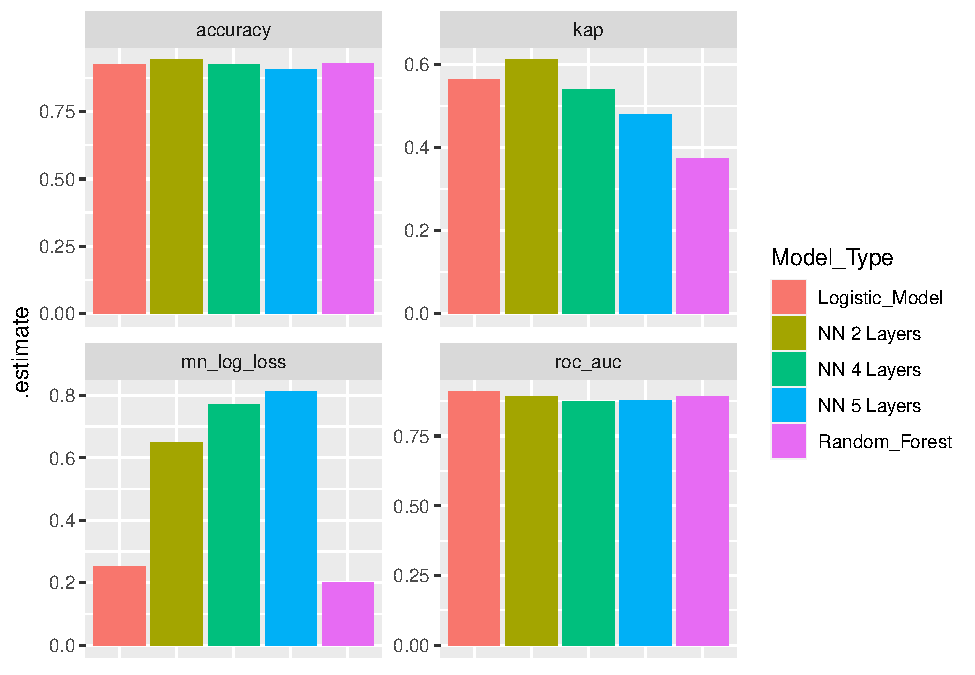
\includegraphics{Project-5-MTW_files/figure-latex/unnamed-chunk-16-1.pdf}

As we can see, the two main metrics, accuracy and auc don't vary
greatly, but they do vary. Interestingly the logistic and the random
forest models performed the best, with all three neural nets performing
somewhat worse.

This is likely due to the massive amount of options that are available
when tuning a neural net. Looking at efficient parameter tuning (such as
the methods used for the other two models) may be a worthwhile effort.

Another possibility is that the upsampling led to decreased accuracy
only because the test data set was so imbalanced. An analysis of
precision vs recall could be worthwhile. Perhaps we are willing to
sacrifice some misclassification of the majority class if it means we
more accurately predict the minority class.

\end{document}
